\documentclass[tikz,border=5pt]{standalone}
\begin{document}
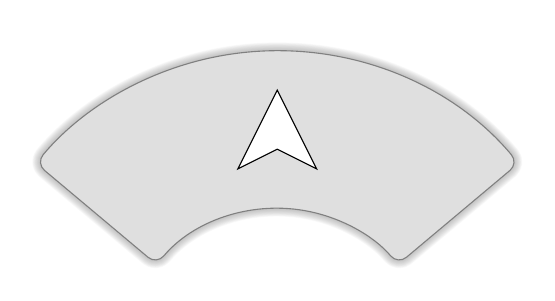
\begin{tikzpicture}[
        % https://tex.stackexchange.com/a/569645
        myglow/.style={%
            preaction={#1, draw, line join=round, line width=0.5pt, opacity=0.05,
            preaction={#1, draw, line join=round, line width=1.0pt, opacity=0.05,
            preaction={#1, draw, line join=round, line width=1.5pt, opacity=0.05,
            preaction={#1, draw, line join=round, line width=2.0pt, opacity=0.05,
            preaction={#1, draw, line join=round, line width=2.5pt, opacity=0.05,
            preaction={#1, draw, line join=round, line width=3.0pt, opacity=0.05,
            preaction={#1, draw, line join=round, line width=3.5pt, opacity=0.05,
            preaction={#1, draw, line join=round, line width=4.0pt, opacity=0.05,
            preaction={#1, draw, line join=round, line width=4.5pt, opacity=0.05,
            preaction={#1, draw, line join=round, line width=5.0pt, opacity=0.05,
            preaction={#1, draw, line join=round, line width=5.5pt, opacity=0.05,
            preaction={#1, draw, line join=round, line width=6.0pt, opacity=0.05,
        }}}}}}}}}}}}}
    ]
  \draw[
    fill=gray!25,
    draw=gray,rounded corners,
    myglow=gray,
    ]
    (40:4)
    arc[start angle=40,end angle=140,radius=4] 
    -- (140:2)
    arc[start angle=140,end angle=40,radius=2] 
    -- cycle;
    \draw[fill=white] (0,2.75) -- ++(.5,-.25) -- (0,3.5) -- ++(-.5,-1) -- cycle;
\end{tikzpicture}
\end{document}
